\chapter{Architecture and Implementation}

\section{System Architecture Overview}
The proposed serverless architecture is designed to prioritize both rigorous workload isolation and near-zero invocation latency. To achieve this, we synthesize several established open-source technologies: \texttt{containerd}, \texttt{nerdctl}, Kata Containers, and QEMU. The core innovation lies not in the individual components, but in their orchestration to implement a persistent, paused "warm pool" of microVMs.

Figure \ref{fig:arch} illustrates the high-level architecture of the system.

\begin{figure}[h]
    \centering
    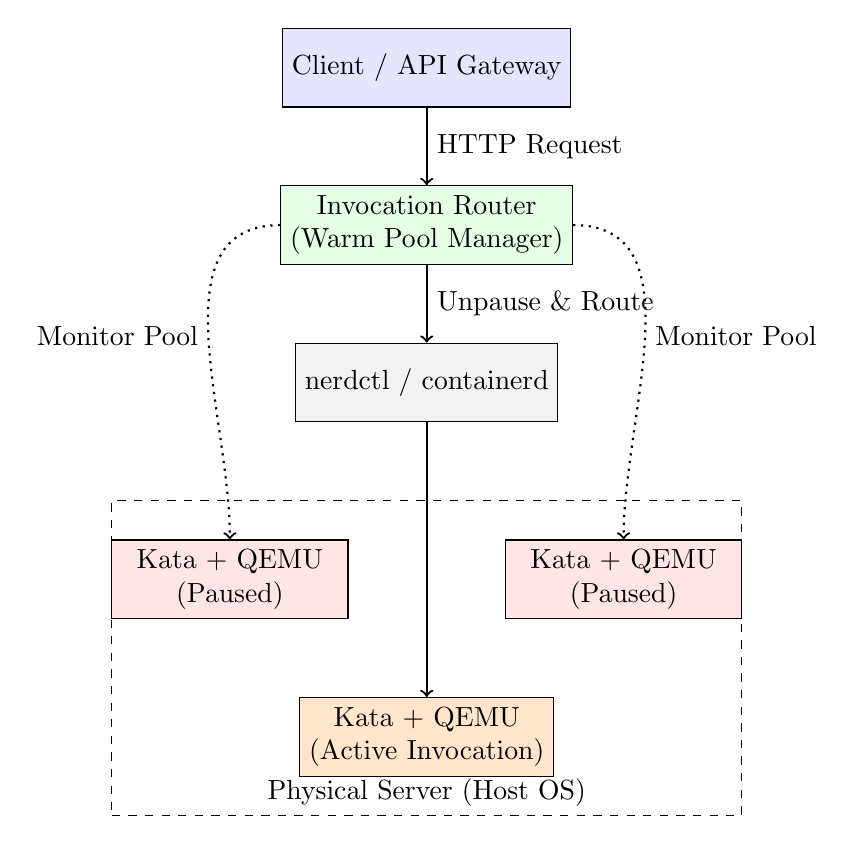
\begin{tikzpicture}[
        box/.style={draw, rectangle, minimum width=3cm, minimum height=1cm, align=center},
        arrow/.style={->, thick}
    ]
        % Nodes
        \node[box, fill=blue!10] (client) at (0, 0) {Client / API Gateway};
        \node[box, fill=green!10] (router) at (0, -2) {Invocation Router\\(Warm Pool Manager)};

        \node[box, fill=gray!10] (nerdctl) at (0, -4) {nerdctl / containerd};

        \node[box, dashed, minimum width=8cm, minimum height=4cm, label={[anchor=south]south:Physical Server (Host OS)}] (host) at (0, -7.5) {};

        \node[box, fill=red!10] (kata1) at (-2.5, -6.5) {Kata + QEMU\\(Paused)};
        \node[box, fill=red!10] (kata2) at (2.5, -6.5) {Kata + QEMU\\(Paused)};
        \node[box, fill=orange!20] (kata3) at (0, -8.5) {Kata + QEMU\\(Active Invocation)};

        % Arrows
        \draw[arrow] (client) -- node[right] {HTTP Request} (router);
        \draw[arrow] (router) -- node[right] {Unpause \& Route} (nerdctl);
        \draw[arrow] (nerdctl) -- (kata3);
        \draw[arrow, dotted] (router) to[out=180,in=90] node[left] {Monitor Pool} (kata1);
        \draw[arrow, dotted] (router) to[out=0,in=90] node[right] {Monitor Pool} (kata2);

    \end{tikzpicture}
    \caption{High-Level Architecture of the Warm-MicroVM Serverless Platform}
    \label{fig:arch}
\end{figure}

\section{Component Roles}

\subsection{Containerd and Nerdctl}
\texttt{containerd} serves as the industry-standard core container runtime. It manages the complete container lifecycle of its host system, from image transfer and storage to container execution and supervision.
In our architecture, we utilize \texttt{nerdctl}, a Docker-compatible command-line interface for containerd. \texttt{nerdctl} is chosen over standard Docker due to its cutting-edge feature support (such as native IPFS integration and experimental rootless modes) and its seamless, low-level integration directly with containerd namespaces. It allows us to manage containers and their states (start, stop, pause, unpause) with minimal overhead.

\subsection{Kata Containers and QEMU}
While containerd handles the OCI-compliant management, the actual execution is delegated to Kata Containers. Kata configures the runtime environment not as a standard Linux namespace, but as a dedicated Virtual Machine.
For the hypervisor, we utilize QEMU. QEMU is a highly mature, generic, and open-source machine emulator and virtualizer. When used in conjunction with KVM (Kernel-based Virtual Machine), QEMU provides near-native performance for hardware virtualization. Kata instructs QEMU to boot a minimal guest kernel, optimized specifically for running containers.
The combination of Kata and QEMU provides the necessary security boundary: a kernel panic or container escape within a serverless function only compromises the lightweight Kata VM, leaving the host infrastructure and other functions secure.

\section{Implementing the Warm-Up Strategy}

The crux of the implementation is mitigating the boot time of the QEMU virtual machine. Traditional serverless platforms boot the VM upon receiving a request (cold start). Our architecture employs a "Warm Pool" manager.

\subsection{Pre-Provisioning}
During system initialization or during periods of low load, the Warm Pool Manager uses \texttt{nerdctl} to preemptively spin up instances of the serverless runtime image.
\begin{minted}{bash}
# Example command to start a Kata container in the background
nerdctl run -d --runtime=io.containerd.kata.v2 --name function_vm_1 serverless-base-image
\end{minted}

\subsection{Pausing State}
Once the container and its underlying QEMU VM are fully booted and the application server within is listening, the state is immediately frozen.
\begin{minted}{bash}
# Pause the container execution
nerdctl pause function_vm_1
\end{minted}
At the hypervisor level, pausing a container via \texttt{containerd/nerdctl} translates to suspending the virtual CPUs of the QEMU process via cgroups. A paused VM consumes resident memory but requires strictly zero CPU cycles. It sits completely dormant.

\subsection{Invocation and Unpausing}
When an HTTP request arrives for a serverless function, the Invocation Router intercepts it.
\begin{enumerate}
    \item \textbf{Selection:} The router selects an available paused VM from the pool (\texttt{function\_vm\_1}).
    \item \textbf{Unpause:} The router issues a command to resume execution.
    \begin{minted}{bash}
nerdctl unpause function_vm_1
    \end{minted}
    Unpausing is an extremely fast operation, typically requiring less than 5 milliseconds, as it simply involves lifting the cgroup CPU restrictions. The guest OS does not need to boot; it resumes execution instantly from where it was suspended.
    \item \textbf{Execution:} The HTTP request is forwarded to the now-active container, which executes the function payload.
    \item \textbf{Recycling:} After execution, the container environment can be cleansed and paused again to rejoin the warm pool, or destroyed and replaced by a fresh pre-provisioned instance to guarantee absolute state immutability between invocations.
\end{enumerate}

\section{Security Considerations}
By leveraging Kata Containers, every function invocation is isolated by hardware virtualization boundaries. The warm pool strategy does not compromise this isolation. Because the pre-provisioned image only contains the generic serverless runtime, user-specific function code is only injected \textit{after} the VM is unpaused and allocated to a specific tenant. This ensures that no cross-tenant state leakage can occur within the warm pool itself.

\vspace{2cm}
\lipsum[41-60] % Dummy text for length
